\chapter{SỬ DỤNG CÁC BIỂU ĐỒ}
\label{chap:bieudo}


\section{Giới thiệu về biểu diễn bằng đồ thị}
\label{sec:dothi}
Trong rất nhiều lĩnh vực cần phải trình bày, giới thiệu các thông tin liên quan tới con số, thống kê hay các dữ liệu khác. Các dữ liệu đo đạc, tính toán thường được thu thập dưới dạng bảng biểu; tuy nhiên bảng biểu chỉ thích hợp khi trình bày các số lượng nhỏ các số liệu, đồng thời không cung cấp các đánh giá trực quan về xu hướng của dữ liệu thu được.

Đồ thị có khả năng cung cấp hình ảnh trực quan, dễ hiểu giúp người đọc nhanh chóng nắm bắt được ý tưởng muốn nhấn mạnh, muốn trình bày. Người trình bày cần lựa chọn đúng loại đồ thị và không nên sử dụng các đồ thị quá màu mè; lựa chọn tên đồ thị ngắn gọn, dễ hiểu. Các loại đồ thị thường gặp là:
\begin{itemize}
	\item[-] Kiểu bánh (Pie charts)
	\item[-] Kiểu thanh ngang \& dọc (kiểu cột) (Horizontal \& Vertical bar charts)
	\item[-] Kiểu đường \& Kiểu phân bố (Line charts \& Scatter diagrams)
	\item[-] Kiểu diện tích (Area charts)
\end{itemize}

\begin{figure}[h]
\centering
	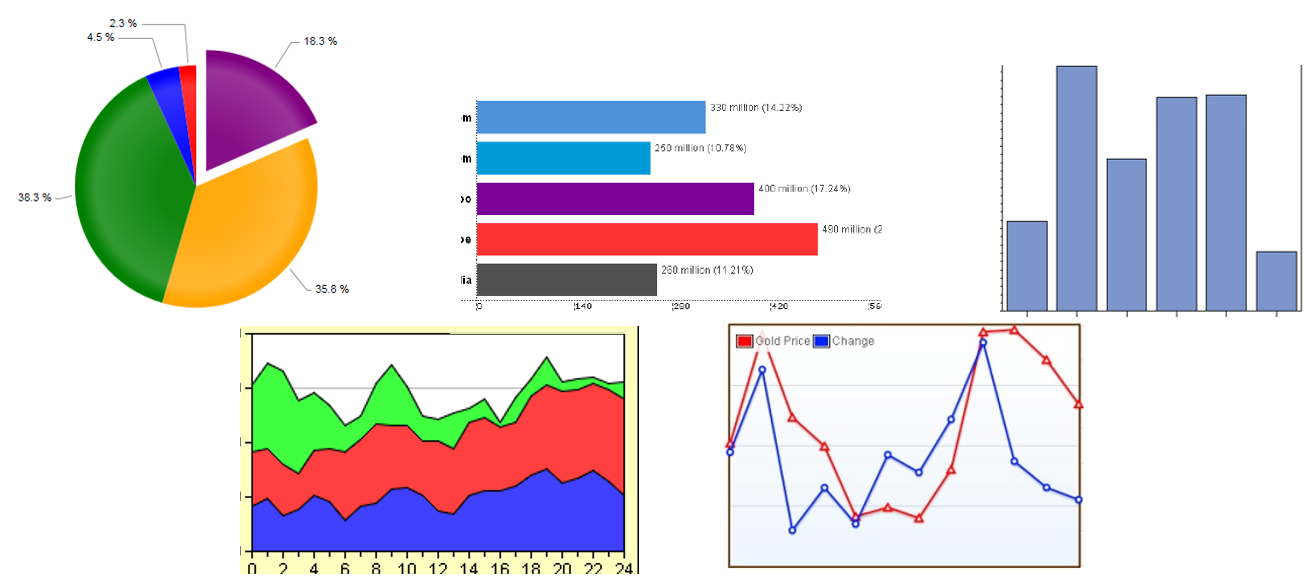
\includegraphics[scale=0.4]{figures/fig4}
\end{figure}

Phần tiếp theo sẽ khuyến cáo về phạm vi sử dụng của từng loại đồ thị này.
\section{Đồ thị kiểu bánh}
\label{sec:banh}
Phạm vi sử dụng:
\begin{itemize}
	\item[-] Dùng để biểu thị tỷ lệ phần trăm (\%)
	\item[-] Biểu diễn mối liên hệ tương quan tỷ lệ
	\item[-] Không nên dùng quá nhiều miếng (tối đa 6 miếng) trong một đồ thị
\end{itemize}
\begin{figure}[h]
\centering
	
\includegraphics[scale=0.5]{figures/fig5}
\end{figure}
Khi muốn nhấn mạnh một đại lượng:
\begin{itemize}
 \item[-] Để diễn tả phần quan trọng: đặt phần quan trọng này ở phía trên, bên phải, tính từ vị trí 1 giờ
 \item[-] Khi cần nhấn mạnh: có thể kéo phần nhô này ra khỏi đồ thị ( nhấn mạnh về tỷ trọng phần trăm của ngô là nhỏ nhất)
\end{itemize}

\begin{figure}[h]
\centering
	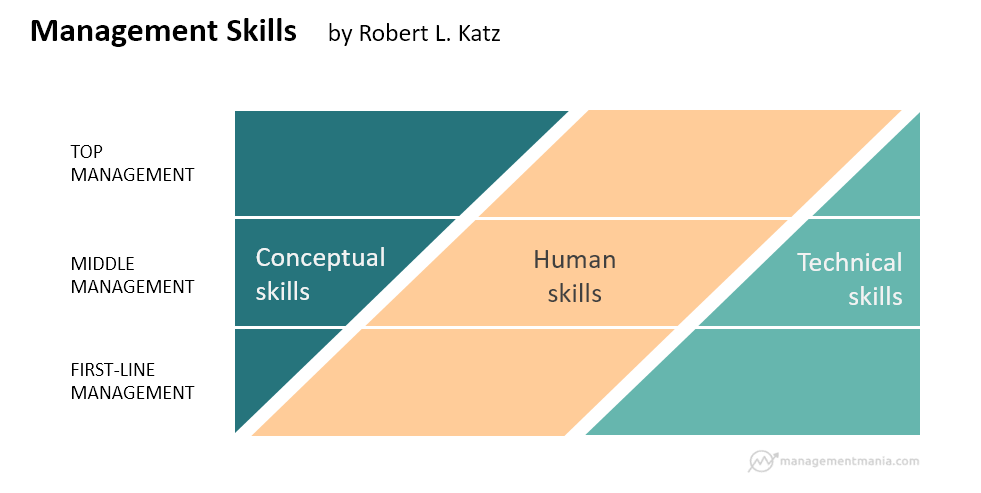
\includegraphics[scale=0.5]{figures/fig6}
\end{figure}

\section{Đồ thị kiểu thanh ngang}
\label{sec:thanhngang}

\section{Đồ thị kiểu cột đứng}
\label{sec:cotdung}

\section{Đồ thị kiểu diện tích}
\label{sec:dientich}
